\section{Concepts and language support}

To provide a design-time support for building adaptive software that change its
behavior depending on the situation, we introduce two main notions:
\emph{i)} individual \emph{context} and \emph{ii) context group}, whose along
with a number of secondary notions form a complete design. The latter helps to
to identify the common functionality, orthogonal aspects and mutual constraints.
Context represents an environmental situation the system may find itself in, and
defines a behavioral variation. The software adapts to the
environmental dynamics by \emph{activating} the corresponding context. Context
groups represent the collections of contexts and combines the behavior
variations of the same functionality.

\begin{figure}
\begin{center}
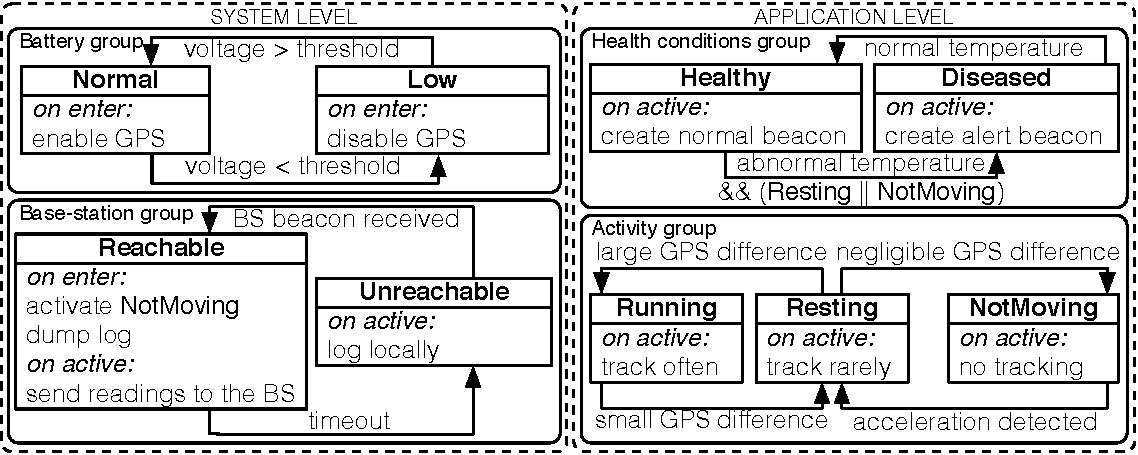
\includegraphics[scale=.45]{imgs/wildlifetracking}
\vspace{-1mm}
\caption{Wildlife monitoring application design.}
  \label{fig:design}
\vspace{-9mm}
\end{center}
\end{figure}

{\bf \conesc.} To be more concrete in our design, we render the concepts above in
a set of language constructs, according to a context-oriented programming
(COP)~\cite{Hirschfeld08}. Our target language nesC -- one of the most popular
for programming for WSNs derived from C -- exemplifies the restrictions of CPSs
such as limited memory and CPU performance as well as absence of memory
protection. Applications in nesC are built from \emph{components} interconnected
by \emph{configuration} and interacted by \emph{using} and \emph{providing}
interfaces. The latter define two types of functions: \emph{commands} and
\emph{events}. The components can not be instantiated at run-time, and dynamic
allocation is also discouraging. Taking into account restrictions above, we
developed a context-oriented extension of nesC language, called \conesc.

The context-oriented design of our motivating example is displayed in
Fig.~\ref{fig:design}. Context groups describe a behavioral variation
corresponding to battery level, base-station availability, health conditions and
activity of an animal. Notion of \emph{context group} allows us to separate
re-usable system services from application-specific functionality. In \conesc
\emph{context group} extends a standard nesC configuration by following
key-words: \code{contexts} to specify included contexts, \code{layered} to
declare layered functions -- the core notion of COP~\cite{Hirschfeld08} meant to
implement a behavioral variation -- \code{is default} to define the active
context at start-up, and optional modifier \code{is error} to specify an error
context. The latter is automatically activated should the constraints be
violated, e.g., when "Diseased'' is activated, "Resting'' or "NotMoving'' must
be active, as shown in Figure~\ref{fig:design}. Explicit context activation can
be initiated anywhere in the code:

\vspace{-1mm}
\begin{lstlisting}[language=conesc]
activate BaseStationG.Unreachable;
\end{lstlisting}
\vspace{-1.5mm}

The context corresponds to the behavioral variation for a given situation. For
example, software behaves differently, depending on whether the base-station is
reachable or not. For example, Figure~\ref{fig:context} shows the \conesc
specification of the "Reachable'' context, which contains an implementation of
behavioral variation -- layered function. The latter represents \emph{continuous
activity} that occurs as long as context is active. For example, software logs
contacts locally as long as "Unreachable'' context is active, as it is
implemented on line~\lstref{ct:layer} by using a key-word \code{layered}.

Opposite to \emph{continuous activities}, there are also \emph{on-time
operations} executed at the time of entering or exiting a context. For example,
log is dumped on the base-station on entering the context "Ureachable''. These
operations can be implemented by using predefined events \code{activated()} and
\code{deactivated()}, shown on lines~\lstref{ct:activate}
and~\lstref{ct:deactivate}. They are automatically signaled when
entering or leaving the contexts.

The contexts transitions within the group are governed by rules. For example,
within "Base-station'' group, the system initiates the transition from
"Reachable'' to "Unreachable'' whenever there are no beacons are received within
a specific timeout. Contexts indicated after the key-word \code{transitions} on
line \lstref{ct:tr} represents possible outgoing transitions. They are also
possibly followed by a key-word \code{iff} to state constraints on the
transitions, as in

\vspace{-1mm}
\begin{lstlisting}[language=conesc]
transitions Diseased iff Resting || NotMoving;
\end{lstlisting}
\vspace{-1.5mm}

The example is in "Health conditions'' group: when activating "Diseased''
context based on body temperature, the software should also check that either
"NotMoving'' or "Resting'' in "Activity group'' is currently active. Should the
constraints be violated, the error context defined in the corresponding context
group is activated. Indeed, a diseased animal is probably not very active.
Otherwise, developers might have not correctly catch the contexts
evolution.

The required adaptation may affect several context groups. For example, along
with the base-station is "Reachable'', context "NotMoving'' should be also
activated. The latter saves energy by disabling GPS-sensor, since the
base-station is static and deployed in the known location. To this end,
the keyword \code{triggers} on line~\lstref{ct:trigger} binds the activation
across the groups. For example, the context "NotMoving'' is activated on
entering the "Reachable'', as specified in Figure~\ref{fig:design}.


\begin{figure}[!tb]
\begin{lstlisting}[style=conescframe]
context Reachable {
*\lstnote{ct:tr}* transitions Unreachable;
*\lstnote{ct:trigger}* triggers NotMoving;
 uses interface Radio;
} implementation {
*\lstnote{ct:layer}* layered command void report(contact_t contact){
  call Radio.send(contact);}
*\lstnote{ct:activate}* event void activated(){// Dump logs on base-station }
*\lstnote{ct:deactivate}* event void deactivated(){ // Radio clean-up }}
\end{lstlisting}
\caption{Individual context in \conesc.}
  \label{fig:context}
\vspace{-5mm}
\end{figure}
